
\subsection{Sensitivity to Training-Subset Selection and Consistency of Regional Predictions}
\label{subsec:training-selection-sensitivity}

Under limited training data, prediction accuracy can be sensitive to the selection of target-domain samples. Figure~\ref{fig:training-selection-stability} compares the validation errors of M0, M1, and M2 across five different training subsets at $N=20$ and $N=50$. With the network training random seed held fixed, changing the training subset introduces variations in RMSE, while the relative performance of the three knowledge configurations remains consistent. M1 outperforms M0 across all examined subsets, and M2 consistently achieves the lowest errors. For M2, the RMSE ranges from 0.0312 to 0.0374 at $N=20$, narrowing to 0.0242--0.0259 at $N=50$. These results indicate that the accuracy advantage of hierarchical knowledge transfer is maintained across the examined training subsets rather than depending on a particular selection of target-domain samples.

\begin{figure*}[!t]
    \centering
    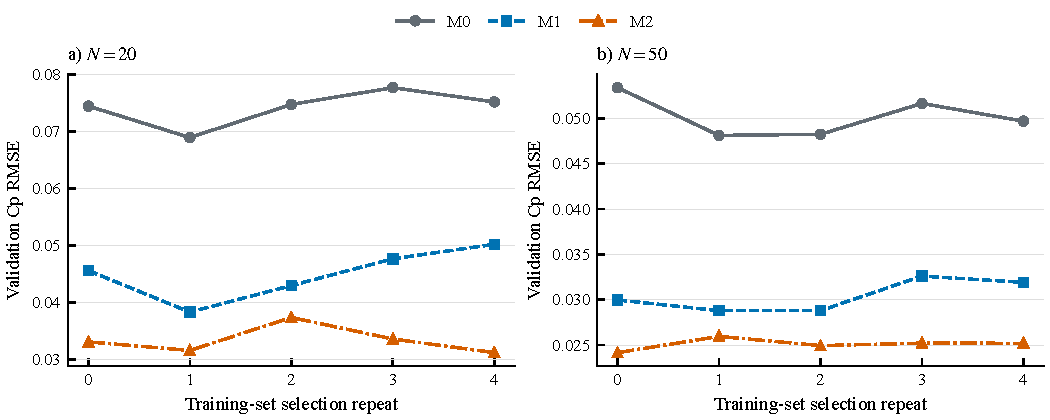
\includegraphics[width=0.93\textwidth]{V_Results_and_Discussion/figures/V_D_Fig23/V_D_Fig23_training_selection_stability.pdf}
    \caption{Training-subset sensitivity of M0, M1, and M2 at $N=20$ and $50$ .}
    \label{fig:training-selection-stability}
\end{figure*}

Although the overall prediction accuracy improves with transferred aerodynamic knowledge, the local benefits vary among individual validation wings. Figure~\ref{fig:regional-error-consistency} presents the mean changes in regional RMSE and the fractions of validation wings exhibiting increased errors at different training sizes. The improvement from M0 to M1 is observed for most validation wings in the midspan and wing-tip regions, while the additional improvement from M1 to M2 is more consistent near the wing root. At $N=10$ and $N=20$, only a small fraction of validation wings exhibit increased root-region errors, indicating that the benefits of wing-root knowledge extend beyond a reduction in the mean regional error.

\begin{figure*}[!t]
    \centering
    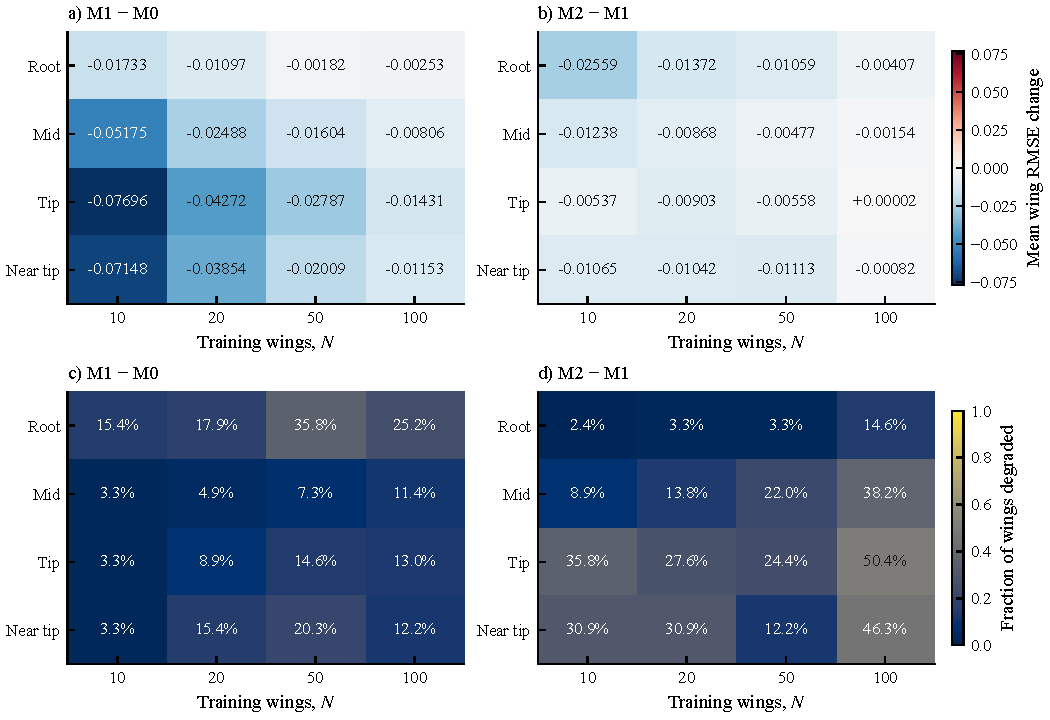
\includegraphics[width=0.95\textwidth]{V_Results_and_Discussion/figures/V_D_Fig24/V_D_Fig24_regional_error_consistency.pdf}
    \caption{Regional RMSE changes and error-increase fractions for M1$-$M0 and M2$-$M1 across four regions and training sizes.}
    \label{fig:regional-error-consistency}
\end{figure*}

As the number of target-domain training samples increases, both the additional benefits of regional knowledge and their consistency across validation wings change. At $N=100$, M2 retains a mean accuracy advantage over M1 in the wing-root region, whereas the additional improvements in the midspan and wing-tip regions become considerably smaller. In particular, the mean RMSE difference in the wing-tip region approaches zero. It should be noted that the fraction of wings exhibiting increased errors reflects only the direction of the paired error changes, rather than their magnitude. Small numerical differences should therefore not be interpreted as substantial prediction degradation. Overall, hierarchical knowledge transfer maintains its accuracy advantage across different training-subset selections, although the consistency of local improvements depends on spanwise location and the availability of target-domain training data.
